
\def\ft{Algoritmos de hashing}

\begin{frame}[fragile]
  \frametitle{\ft}
  \begin{block}{Definición y actores}
    \begin{itemize}
    \item Dado un dato de tamaño arbitrario produce un resumen de N bits
    \item Las garantías del resumen tienen diversos niveles:
      dispersión, dificultad de colisión, uso criptográfico
    \item Multitud de actores con variantes
      CRC32,
      Adler,
      MurmurHash (1, 2 y 3),
      xxHash (XXH32, XXH64, XXH3\_64, XXH3\_128),
      CityHash,
      MetroHash,
      SipHash,
      ...
    \item Siempre trabajan igual
      \begin{itemize}
      \item Descomponen la entrada en bloques de tamaño fijo + una cola
      \item Procesan los bloques secuencialmente
      \item Hay un proceso de cierre, en el que suele intervenir la longitud
        total, y que produce el resumen
      \end{itemize}
    \end{itemize}
  \end{block}
\end{frame}

\begin{frame}[fragile]
  \frametitle{\ft}
  \begin{block}{Planteamientos usuales: hashing para diversos tipos}
    \begin{lstlisting}[language=java]
public interface Hashing {
  long hash(byte x);
  long hash(char x);
  long hash(short x);
  long hash(int x);
  long hash(long x);
  long hash(float x);
  long hash(double x);

  long hash(byte[] xs);
  long hash(byte[] xs, int off, int len);

  long hash(char[] xs);
  long hash(char[] xs, int off, int len);
  long hash(String xs);
  long hash(String xs, int off, int len);
}
    \end{lstlisting}
  \end{block}
\end{frame}

\begin{frame}[fragile]
  \frametitle{\ft}
  \begin{block}{Planteamientos usuales: hashing incremental}
    \begin{lstlisting}[language=java]
public interface Hasher {
  Hasher add(byte x);
  Hasher add(char x);
  Hasher add(short x);
  Hasher add(int x);
  Hasher add(long x);
  Hasher add(float x);
  Hasher add(double x);
  Hasher add(byte[] xs);
  Hasher add(byte[] xs, int off, int len);
  Hasher add(char[] xs);
  Hasher add(char[] xs, int off, int len);
  Hasher add(String xs);
  Hasher add(String xs, int off, int len);

  long hash64();
  int hash(long[] h);
}
    \end{lstlisting}
  \end{block}
\end{frame}

\begin{frame}[fragile]
  \frametitle{\ft}
  \begin{block}{Los {\tt Hasher} se implementan usualmente con un buffer}
    \begin{lstlisting}[language=java]
public class AbstractHasher implements Hasher {
  private byte[] buf;
  private int used;

  protected AbstractHasher() {
    this.buf = new byte[BLOCK_SIZE+7];
    this.used = 0;
  }
  ...
  public Hasher add(int x) {
    Bits.le32(buf, used, x);
    used += 4;
    mayFlush();
    return this;
  }
  ...
}
    \end{lstlisting}
  \end{block}
\end{frame}


\begin{frame}[fragile]
  \frametitle{\ft}
  \begin{block}{¿Cómo se implementa un {\tt Hashing}?}
    \begin{itemize}
    \item A través de un Hasher, salvo para {\tt byte[]}
      (\href{https://github.com/google/guava/blob/master/guava/src/com/google/common/hash/AbstractHashFunction.java}{Guava})
    \item Especializando el código del algoritmo a mano para cada tipo
      (\href{https://github.com/OpenHFT/Zero-Allocation-Hashing/blob/ea/src/main/java/net/openhft/hashing/XxHash.java}{Zero-Allocation-Hashing})
    \end{itemize}
  \end{block}
\end{frame}


\begin{frame}[fragile]
  \frametitle{\ft}
  \begin{block}{Hashish: el experimento fumeta}
    \begin{itemize}
    \item Hashish es una librería de hashing que intenta congujar
      (1) un diseño con descomposición de responsabilidades
      con (2) el mejor rendimiento posible en Java
    \item Para ello se basa fuertemente en Scalar Replacement
    \item Introduce el concepto de {\tt Kernel}
    \end{itemize}
  \end{block}
\end{frame}


\begin{frame}[fragile]
  \frametitle{\ft}
  \begin{block}{Hashish: Un kernel para cada tamaño de bloque}
    \begin{lstlisting}[language=java]
public interface Kernel64 {
  void block(long block);
  void tail(long tail, int taillen, long total);
}

public interface Kernel128 {
  void block(long b0, long b1);
  void tail(long b0, long b1, int taillen, long total);
}
    \end{lstlisting}
  \end{block}
\end{frame}


\begin{frame}[fragile]
  \frametitle{\ft}
  \begin{block}{Hashish: Los kernels se crean a cascoporro}
    \begin{lstlisting}[language=java]
public abstract class HashingKernel64 implements Hashing {
  protected abstract Kernel64 newKernel();
  public long hash(byte x) {
    return integral(Bits.ubyte(x), 1);
  }
  ...
  private long integral(long x, int taillen) {
    Kernel64 kernel = newKernel();
    kernel.tail(x, taillen, taillen);
    return kernel.hash();
  }
  public long hash(long x) {
    Kernel64 kernel = newKernel();
    kernel.block(x);
    kernel.tail(0, 0, 8);
    return kernel.hash();
  }
  ...
    \end{lstlisting}
  \end{block}
\end{frame}


\begin{frame}[fragile]
  \frametitle{\ft}
  \begin{block}{Hashish: Los kernels se crean a cascoporro 2}
    \begin{lstlisting}[language=java]
  ...

  public long hash(byte[] xs, int off, int len) {
    final int W = 8;
    final Kernel64 kernel = newKernel();
    final int blockno = len / W;
    for (int i = 0; i < blockno; i++) {
      kernel.block(Bits.le64(xs, off + W*i));
    }
    final int taillen = len - W*blockno;
    kernel.tail(Bits.le64tail(xs, off + W*blockno, taillen), taillen, len);
    return kernel.hash();
  }
}
    \end{lstlisting}
  \end{block}
\end{frame}


\begin{frame}[fragile]
  \frametitle{\ft}
  \begin{block}{Hashish: Para un nuevo algoritmo basta un nuevo Kernel}
    \begin{lstlisting}[language=java]
public class SipHashKernel implements Kernel64 {
  private long v0, v1, v2, v3;

  public void block(long block) {
    v3 ^= block;
    compressionRounds();
    v0 ^= block;
  }

  public void tail(long tail, int taillen, long totallen) {
    final long mask = ~((~0L) << (8*taillen));
    block((mask & tail) | ((totallen & 0xFF) << 56));
    v2 ^= 0xFF;
    finalizationRounds();
  }
  ...
}
    \end{lstlisting}
  \end{block}
\end{frame}


\begin{frame}[fragile]
  \frametitle{\ft}
  \begin{block}{Hashish: ... y definir el Hashing}
    \begin{lstlisting}[language=java]
public class SipHashing extends HashingKernel64 {
  private final long k0, k1;

  public SipHashing(long k0, long k1) {
    this.k0 = k0;
    this.k1 = k1;
  }

  protected SipHashKernel newKernel() {
    return new SipHashKernel(k0,k1);
  }
}
    \end{lstlisting}
  \end{block}
\end{frame}


\begin{frame}[fragile]
  \frametitle{\ft}
  \begin{block}{Rendimiento sobre byte[3]}
    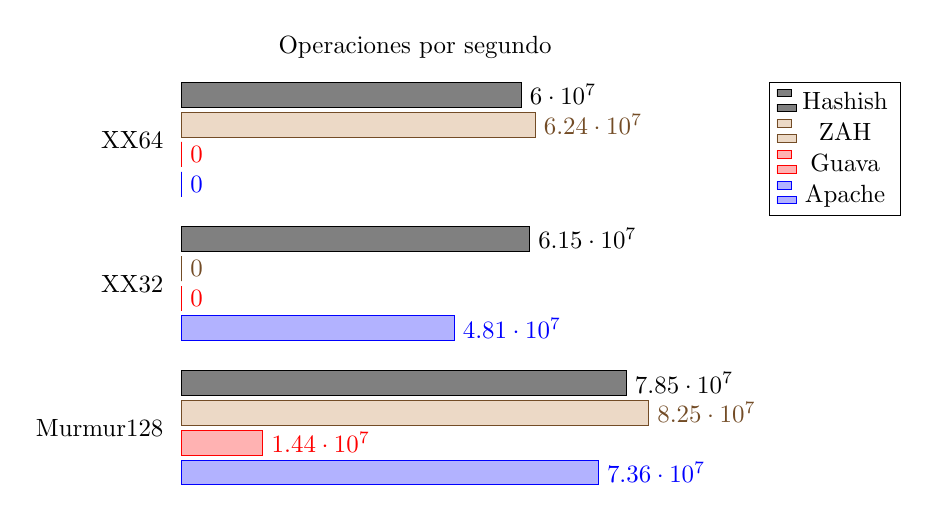
\begin{tikzpicture}[scale=0.9]
      \begin{axis}[
          title  = Operaciones por segundo,
          xbar,
          xmin=0,
          y axis line style = { opacity = 0 },
          axis x line       = none,
          tickwidth         = 0pt,
          enlarge y limits  = 0.2,
          enlarge x limits  = 0.02,
          symbolic y coords = {Murmur128, XX32, XX64},
          ytick=data,
          nodes near coords,
          reverse legend,
          %legend pos=north east,
          legend style={at={(1.5,1)}, anchor=north east},
        ]
        % apache
        \addplot coordinates {
          (73589373.939,Murmur128)
          (48119911.412,XX32)
          (0,XX64)
        };
        % guava
        \addplot coordinates {
          (14371913.397,Murmur128)
          (0,XX32)
          (0,XX64)
        };
        % ZAH
        \addplot coordinates {
          (82480222.390,Murmur128)
          (0,XX32)
          (62431785.506,XX64)
        };
        % Hashish
        \addplot coordinates {
          (78525118.804,Murmur128)
          (61452279.610,XX32)
          (59960144.582,XX64)
        };
        \legend{Apache, Guava, ZAH, Hashish}
      \end{axis}
    \end{tikzpicture}
  \end{block}
\end{frame}


\begin{frame}[fragile]
  \frametitle{\ft}
  \begin{block}{Rendimiento sobre byte[31]}
    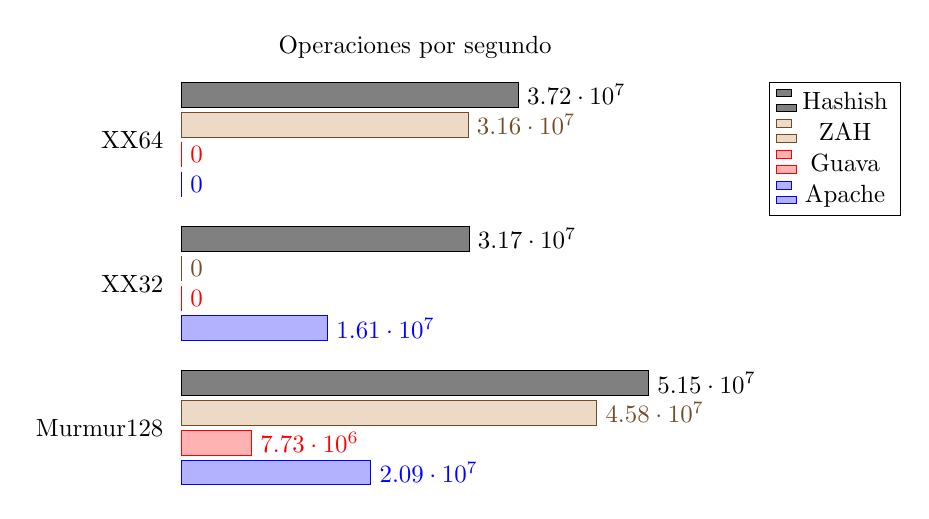
\begin{tikzpicture}[scale=0.9]
      \begin{axis}[
          title  = Operaciones por segundo,
          xbar,
          xmin=0,
          y axis line style = { opacity = 0 },
          axis x line       = none,
          tickwidth         = 0pt,
          enlarge y limits  = 0.2,
          enlarge x limits  = 0.02,
          symbolic y coords = {Murmur128, XX32, XX64},
          ytick=data,
          nodes near coords,
          reverse legend,
          %legend pos=north east,
          legend style={at={(1.5,1)}, anchor=north east},
        ]
        % apache
        \addplot coordinates {
          (20866076.290,Murmur128)
          (16107110.585,XX32)
          (0,XX64)
        };
        % guava
        \addplot coordinates {
          (7734910.459,Murmur128)
          (0,XX32)
          (0,XX64)
        };
        % ZAH
        \addplot coordinates {
          (45790062.374,Murmur128)
          (0,XX32)
          (31611002.009,XX64)
        };
        % Hashish
        \addplot coordinates {
          (51503941.311,Murmur128)
          (31723083.396,XX32)
          (37151254.934,XX64)
        };
        \legend{Apache, Guava, ZAH, Hashish}
      \end{axis}
    \end{tikzpicture}
  \end{block}
\end{frame}


\begin{frame}[fragile]
  \frametitle{\ft}
  \begin{block}{Rendimiento sobre byte[1048607]}
    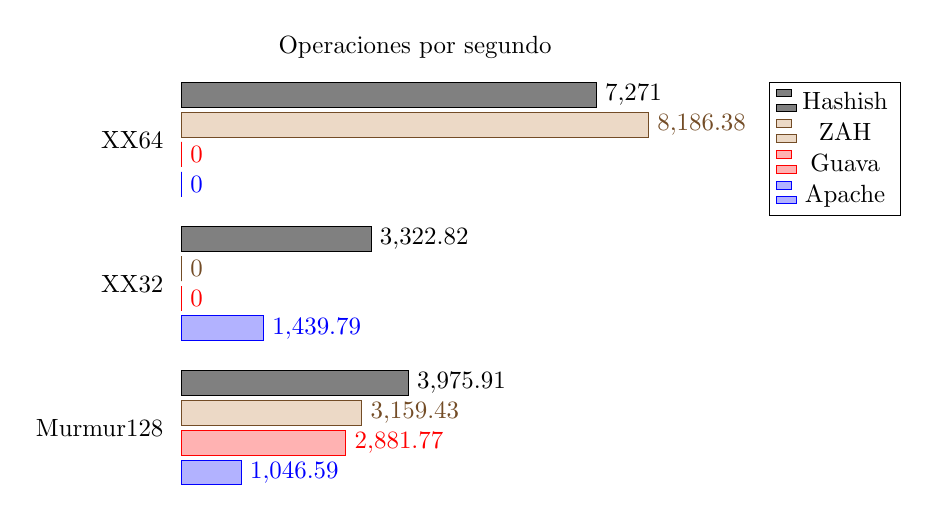
\begin{tikzpicture}[scale=0.9]
      \begin{axis}[
          title  = Operaciones por segundo,
          xbar,
          xmin=0,
          y axis line style = { opacity = 0 },
          axis x line       = none,
          tickwidth         = 0pt,
          enlarge y limits  = 0.2,
          enlarge x limits  = 0.02,
          symbolic y coords = {Murmur128, XX32, XX64},
          ytick=data,
          nodes near coords,
          reverse legend,
          %legend pos=north east,
          legend style={at={(1.5,1)}, anchor=north east},
        ]
        % apache
        \addplot coordinates {
          (1046.593,Murmur128)
          (1439.794,XX32)
          (0,XX64)
        };
        % guava
        \addplot coordinates {
          (2881.766,Murmur128)
          (0,XX32)
          (0,XX64)
        };
        % ZAH
        \addplot coordinates {
          (3159.433,Murmur128)
          (0,XX32)
          (8186.380,XX64)
        };
        % Hashish
        \addplot coordinates {
          (3975.910,Murmur128)
          (3322.824,XX32)
          (7271.002,XX64)
        };
        \legend{Apache, Guava, ZAH, Hashish}
      \end{axis}
    \end{tikzpicture}
  \end{block}
\end{frame}
